\documentclass{article}
\usepackage[utf8]{inputenc}

\usepackage{graphicx,caption}
\graphicspath{ {./images/} }
\usepackage{float}
\usepackage{caption}
\usepackage{subcaption}
\usepackage[unicode]{hyperref}
\usepackage{amsmath}
\usepackage[shortlabels]{enumitem}

\title{Homework 3 - Theory}
\author{Dainese Fabio, 857661}
\date{March 22, 2020}

\begin{document}

\maketitle

\section{Exercise 1}
    \begin{figure}[H]
        \centering
        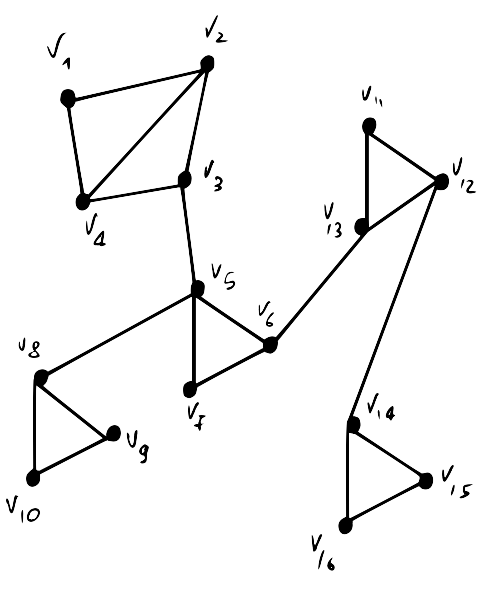
\includegraphics[width=0.5\textwidth]{1.png}
        \caption{Graph \(G=(V,E)\)}
        \label{fig:figure-1}
    \end{figure}
    
    \begin{enumerate}[a)] 
        \item The \textit{clique number} of \(G\) is \(w(G) = 3\). This also means that the \textit{chromatic number} (\(c(G)\)) has a lower bound of:
        \begin{align*}
            c(G) &\geq w(G) \\
            c(G) &\geq 3
        \end{align*}
        
        \item The \textit{max degree} of \(G\) is \(\triangle(G) = max\{d(V) | v \in V\} = 4\). This also means that the \textit{chromatic number} (\(c(G)\)) has a upper bound of:
        \begin{align*}
            c(G) &\leq \triangle(G)+1 \\
            c(G) &\leq 5
        \end{align*}
    \end{enumerate}
    
    \begin{figure}[H]
        \centering
        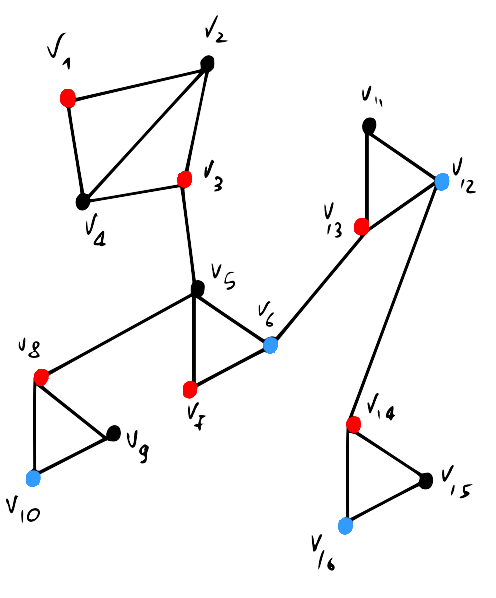
\includegraphics[width=0.5\textwidth]{2.png}
        \caption{Graph \(G=(V,E)\)}
        \label{fig:figure-2}
    \end{figure}
    
    \begin{enumerate}[c)]
        \item The coloring illustrated in the 'Figure \ref{fig:figure-2}' is not a proper 3-colouring of \(G\), since the vertices \(v_{2}\) and \(v_{4}\) are adjacent and with the same color.
        
        \item The partitions of the vertex set induced by the provided colouring are:
        \begin{align*}
            V_{black} &= \{v_{2},v_{4},v_{5},v_{9},v_{11},v_{15},\} \\
            V_{red} &= \{v_{1},v_{3},v_{7},v_{8},v_{13},v_{14},\} \\
            V_{blue} &= \{v_{6},v_{10},v_{12},v_{16},\} \\
        \end{align*}
    \end{enumerate}
    
\section{Exercise 2}
    \begin{figure}[H]
        \centering
        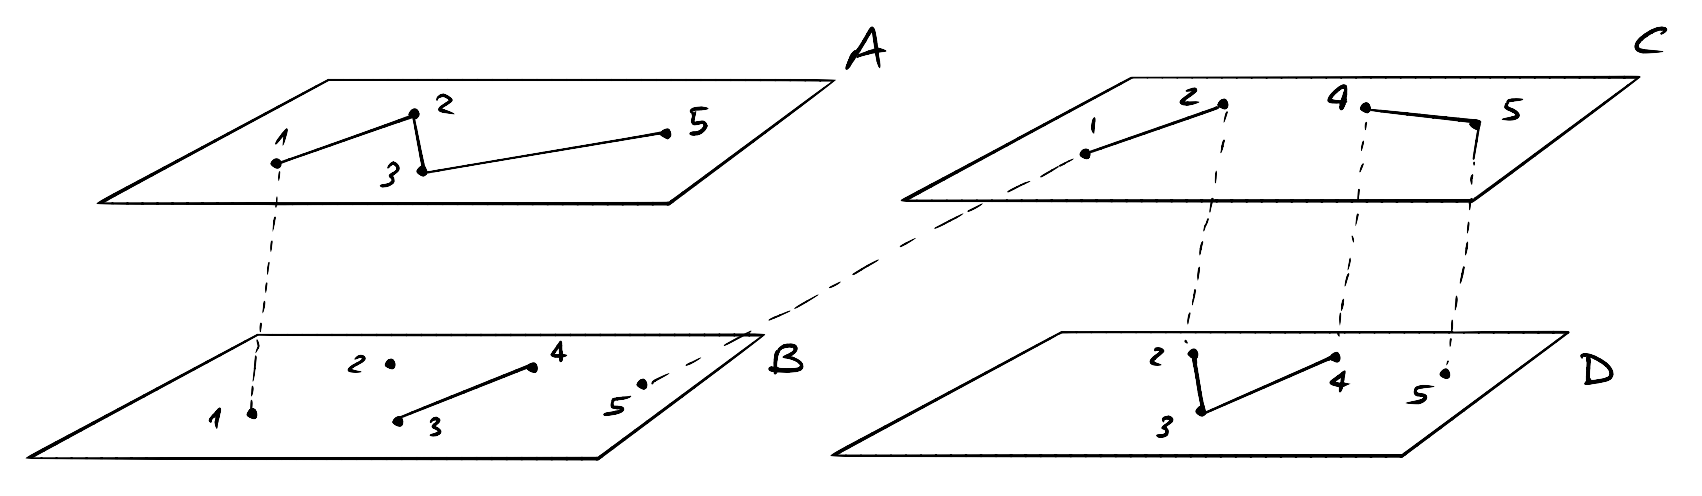
\includegraphics[width=\textwidth]{3.png}
        \caption{Multi-layer network}
        \label{fig:figure-3}
    \end{figure}
    The multi-layer network pictured in the 'Figure \ref{fig:figure-3}' has its vertex and edge sets equals to:
    
    \begin{align*}
        V_{M}=&\{v_{1}=\{1,A\},v_{2}=\{2,A\},v_{3}=\{3,A\},v_{4}=\{5,A\},v_{5}=\{1,B\},v_{6}=\{2,B\},\\
        &v_{7}=\{3,B\},v_{8}=\{4,B\},v_{9}=\{5,B\},v_{10}=\{1,C\},v_{11}=\{2,C\},v_{12}=\{4,C\},\\
        &v_{13}=\{5,C\},v_{14}=\{2,D\},v_{15}=\{3,D\},v_{16}=\{4,D\},v_{17}=\{5,D\}\}
    \end{align*}
    \begin{align*}
        E_{M}=&\{\{v_{1},v_{2}\}, \{v_{2},v_{3}\}, \{v_{3},v_{4}\}, \{v_{1},v_{5}\}, \{v_{7},v_{8}\}, \{v_{9},v_{10}\}, \{v_{10},v_{11}\}, \{v_{12},v_{13}\}, \\ &\{v_{11},v_{14}\}, \{v_{12},v_{16}\}, \{v_{13},v_{17}\}, \{v_{14},v_{15}\}, \{v_{15},v_{16}\}\}
    \end{align*}
    
    \noindent With that said, it also has the following characteristics:
    
    \begin{enumerate}[a)]
        \item Intra-layer edge sets:
        \begin{align*}
            E_{A,A}&=\{\{v_{1},v_{2}\}, \{v_{2},v_{3}\}, \{v_{3},v_{4}\}\} \\
            E_{A,B}&=\{\{v_{7},v_{8}\}\} \\
            E_{A,C}&=\{\{v_{10},v_{11}\},\{v_{12},v_{13}\}\} \\
            E_{A,D}&=\{\{v_{14},v_{15}\},\{v_{15},v_{16}\}\} \\ \\
            E_{A}&= E_{A,A} \cup E_{A,B} \cup E_{A,C} \cup E_{A,D} \\
            &= \{\{v_{1},v_{2}\}, \{v_{2},v_{3}\}, \{v_{3},v_{4}\},\{v_{7},v_{8}\},\\ &\quad\quad\{v_{10},v_{11}\},\{v_{12},v_{13}\},\{v_{14},v_{15}\},\{v_{15},v_{16}\}\}
        \end{align*}
        
        \par\noindent Inter-layer edge sets:
        \begin{align*}
            E_{C,A,B}&=\{\{v_{1},v_{5}\}\} \\
            E_{C,B,C}&=\{\{v_{9},v_{10}\}\} \\
            E_{C,C,D}&=\{\{v_{11},v_{14}\}, \{v_{12},v_{16}\},\{v_{13},v_{17}\}\} \\ \\
            E_{C}&=E_{C,A,B} \cup E_{C,B,C} \cup E_{C,C,D} = E_{M} \setminus E_{A} \\
            &= \{\{v_{1},v_{5}\},\{v_{9},v_{10}\},\{v_{11},v_{14}\}, \{v_{12},v_{16}\}, \{v_{13},v_{17}\}\}
        \end{align*}
        
        \par\noindent Coupling edge set:
        \begin{align*}
            E_{\widetilde{C},A,B}&=\{\{v_{1},v_{5}\}\} \\
            E_{\widetilde{C},C,D}&=\{\{v_{11},v_{14}\}, \{v_{12},v_{16}\}, \{v_{13},v_{17}\}\} \\ \\
            E_{\widetilde{C}}&=E_{\widetilde{C},A,B} \cup E_{\widetilde{C},C,D} \\ &=\{\{v_{1},v_{5}\},\{v_{11},v_{14}\}, \{v_{12},v_{16}\}, \{v_{13},v_{17}\}\}
        \end{align*}
        
        \item The provided network is not \textit{fully interconnected} since not all the layers contain all the nodes.
        
        \item The tensor representation of the network is:
        \begin{align*}
            A_{::,A,A} &= 
            \begin{bmatrix}
            0 & 1 & 0 & 0 & 0 \\
            1 & 0 & 1 & 0 & 0 \\
            0 & 1 & 0 & 0 & 1 \\
            0 & 0 & 0 & 0 & 0 \\
            0 & 0 & 1 & 0 & 0 \\
            \end{bmatrix}\\
            A_{::,B,B} &= 
            \begin{bmatrix}
            0 & 0 & 0 & 0 & 0 \\
            0 & 0 & 0 & 0 & 0 \\
            0 & 0 & 0 & 1 & 0 \\
            0 & 0 & 1 & 0 & 0 \\
            0 & 0 & 0 & 0 & 0 \\
            \end{bmatrix}\\
            A_{::,C,C} &= 
            \begin{bmatrix}
            0 & 1 & 0 & 0 & 0 \\
            1 & 0 & 0 & 0 & 0 \\
            0 & 0 & 0 & 0 & 0 \\
            0 & 0 & 0 & 0 & 1 \\
            0 & 0 & 0 & 1 & 0 \\
            \end{bmatrix}\\
            A_{::,D,D} &= 
            \begin{bmatrix}
            0 & 0 & 0 & 0 & 0 \\
            0 & 0 & 1 & 0 & 0 \\
            0 & 1 & 0 & 1 & 0 \\
            0 & 0 & 1 & 0 & 0 \\
            0 & 0 & 0 & 0 & 0 \\
            \end{bmatrix}\\
            A_{::,A,B} = A_{::,B,A} &= 
            \begin{bmatrix}
            1 & 0 & 0 & 0 & 0 \\
            0 & 0 & 0 & 0 & 0 \\
            0 & 0 & 0 & 0 & 0 \\
            0 & 0 & 0 & 0 & 0 \\
            0 & 0 & 0 & 0 & 0 \\
            \end{bmatrix}\\
            A_{::,B,C} = A_{::,C,B} &= 
            \begin{bmatrix}
            0 & 0 & 0 & 0 & 1 \\
            0 & 0 & 0 & 0 & 0 \\
            0 & 0 & 0 & 0 & 0 \\
            0 & 0 & 0 & 0 & 0 \\
            1 & 0 & 0 & 0 & 0 \\
            \end{bmatrix}\\
            A_{::,C,D} = A_{::,D,C} &= 
            \begin{bmatrix}
            0 & 0 & 0 & 0 & 0 \\
            0 & 1 & 0 & 0 & 0 \\
            0 & 0 & 0 & 0 & 0 \\
            0 & 0 & 0 & 1 & 0 \\
            0 & 0 & 0 & 0 & 1 \\
            \end{bmatrix} 
        \end{align*}
        
        \noindent Just to clarify, the rest of the tensors combinations has not been reported for brevity, since they all are equals to the null matrix.
        
    \end{enumerate} 
    
\section{Exercise 3}
    \begin{figure}[H]
        \centering
        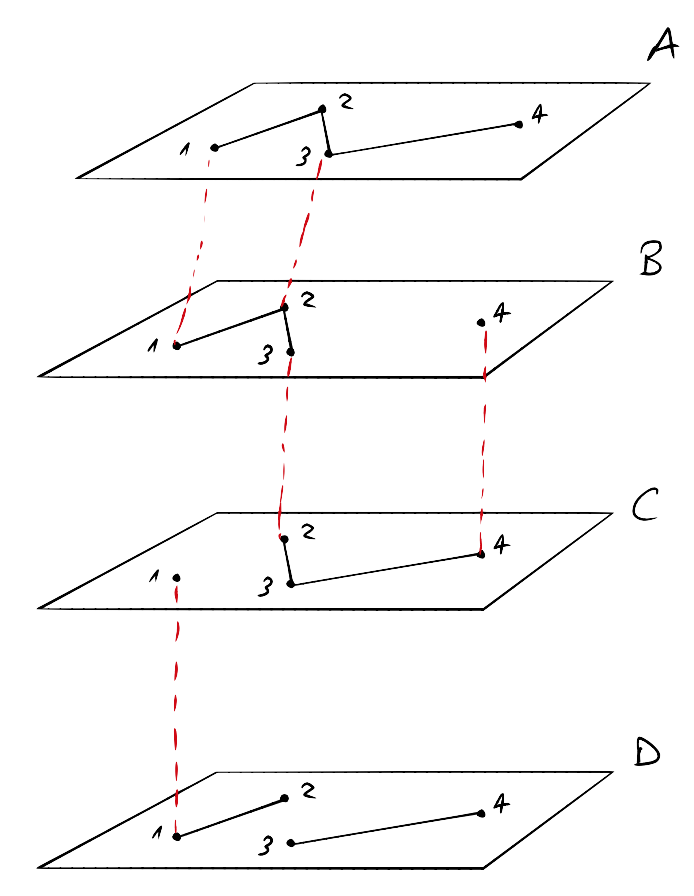
\includegraphics[width=0.6\textwidth]{4.png}
        \caption{Multi-layer graph}
        \label{fig:figure-4}
    \end{figure}
    \begin{enumerate}[a)]
    \item The multi-layer graph pictured in the 'Figure \ref{fig:figure-4}' has the following tensor representation:
    \begin{align*}
            A_{::,A,A} &= 
            \begin{bmatrix}
            0 & 1 & 0 & 0 \\
            1 & 0 & 1 & 0 \\
            0 & 1 & 0 & 1 \\
            0 & 0 & 1 & 0 \\
            \end{bmatrix}\\
            A_{::,B,B} &= 
            \begin{bmatrix}
            0 & 1 & 0 & 0 \\
            1 & 0 & 1 & 0 \\
            0 & 1 & 0 & 0 \\
            0 & 0 & 0 & 0 \\
            \end{bmatrix}\\
            A_{::,C,C} &= 
            \begin{bmatrix}
            0 & 0 & 0 & 0 \\
            0 & 0 & 1 & 0 \\
            0 & 1 & 0 & 1 \\
            0 & 0 & 1 & 0 \\
            \end{bmatrix}\\
            A_{::,D,D} &= 
            \begin{bmatrix}
            0 & 1 & 0 & 0 \\
            1 & 0 & 0 & 0 \\
            0 & 0 & 0 & 1 \\
            0 & 0 & 1 & 0 \\
            \end{bmatrix}\\
            A_{::,A,B} = A_{::,B,A} &= 
            \begin{bmatrix}
            1 & 0 & 0 & 0 \\
            0 & 0 & 1 & 0 \\
            0 & 1 & 0 & 0 \\
            0 & 0 & 0 & 0 \\
            \end{bmatrix}\\
            A_{::,B,C} = A_{::,B,C}&= 
            \begin{bmatrix}
            0 & 0 & 0 & 0 \\
            0 & 0 & 1 & 0 \\
            0 & 1 & 0 & 0 \\
            0 & 0 & 0 & 1 \\
            \end{bmatrix}\\
            A_{::,C,D} = A_{::,D,C} &= 
            \begin{bmatrix}
            1 & 0 & 0 & 0 \\
            0 & 0 & 0 & 0 \\
            0 & 0 & 0 & 0 \\
            0 & 0 & 0 & 0 \\
            \end{bmatrix}\\
    \end{align*}
    
    \noindent As before, the rest of the tensors combinations has not been reported for brevity, since they all are equals to the null matrix.
    
    \item The degree of each node are:
    \begin{align*}
        d_{1} &= (1,1,0,1) \\
        d_{2} &= (2,2,1,1) \\
        d_{3} &= (2,1,2,1) \\
        d_{4} &= (1,0,1,1) \\
    \end{align*}
    
    \par\noindent Meanwhile the overlapping degree are:
    \begin{align*}
        o_{1} &= 3 \\
        o_{2} &= 6 \\
        o_{3} &= 6 \\
        o_{4} &= 3 \\
    \end{align*}
    
    \par\noindent Finally by applying the uniform-vector-like eigenvector centrality we obtain:
    
    \begin{align*}
    \Tilde{A} = A_{::,A,A}^{T} + A_{::,B,B}^{T} + A_{::,C,C}^{T} + A_{::,D,D}^{T} =
        \begin{bmatrix}
            0 & 3 & 0 & 0 \\
            3 & 0 & 3 & 0 \\
            0 & 3 & 0 & 3 \\
            0 & 0 & 3 & 0 \\
        \end{bmatrix}\\
    \end{align*}
    
    \noindent In which every column, and also every row since it's a symmetric matrix, identifies the eigenvector of the relative node (e.g. first row = first column = eigenvector of \(v_{1}\)).
    
    \end{enumerate}

\end{document}
